\documentclass[11pt]{scrartcl}

\usepackage{ucs}
\usepackage[utf8x]{inputenc}
\usepackage[T1]{fontenc}
\usepackage[ngerman]{babel}
\usepackage{amsmath,amssymb,amstext}
\usepackage{graphicx}
\usepackage[justification=RaggedRight, singlelinecheck=false]{caption}
\usepackage{tikz}
\usepackage[square,sort,comma,numbers]{natbib}
\usepackage{url}

\title{Fortgeschrittenen Praktikum Teil 2: PI}
\subtitle{Versuch 1: Hall-Effekt \\ Betreuer: Peter Gruszka}

\author{Gruppe 1: Reinhold Kaiser, Florian Stoll}

\date{04.06.2018}

\begin{document}
\maketitle
\newpage
\tableofcontents
\newpage
\bibliographystyle{alphadin}
\section{Zielsetzung}

\section{Theoretische Grundlagen}
\subsection{Bandstrukturen}
Bandstrukturen in Kristallen sind dadurch zu erklären, dass sich die Atomorbitale der einzelnen Atome überlagern. Aus den diskreten Energieniveaus der einzelnen Atome werden so Energiebänder. Dieses Modell nennt man auch ``tight binding''. Ein anderes Modell genannt ``plane wave expansion'' nimmt an, dass die Elektronen im Kristall quasi frei sind und so durch ausgedehnte Wellen beschrieben werden können. Die Dispersionsrelation wird aber durch die Gitterstruktur verändert und so entstehen Energiebänder, die so Bandlücken in die eigentlich verbundene Energieverteilung bringen.

Anhand der Besetzung dieser Energiebänder lassen sich Materialien in drei unterschiedliche Kategorien bezüglich der Leitfähigkeit einordnen. Denn ein Material leitet nur, wenn das energetisch höchste Energieband nur teilweise besetzt ist. Im Gegensatz zu diesen Metallen haben die Isolatoren zwischen dem letzten besetzten Energieband (Valenzband) und dem nächsten unbesetzten Energieband (Leitungsband) eine Bandlücke, die von den Elektronen normalerweise nicht überwunden werden kann. Bei den Halbleitern ist diese Bandlücke besonders klein, sodass Elektronen beispielsweise durch thermische Anregung in das Leitungsband gelangen können. Die Größe der Energielücken für Halbleiter ist im Bereich von einigen Zehntel eV.

Intrinsische Halbleiter sind Halbleiter, die keine Fehlstellen oder Fremdatome haben und dennoch durch elektronische Anregungen leitfähig werden können. Um nun die Konzentration der Elektronen im Leitungsband zu berechnen nutzt man die Beziehung
\begin{equation}
\frac{N}{V}=n = 2\cdot \int_{E_L}^\infty D_L(E)\cdot f(E)dE
\end{equation}
mit der Fermi-Verteilung $f(E)$ und der Zustandsdichte im Leitungsband $D_L(E)$.
Analog findet man die Beziehung für die Konzentration der Löcher im Valenzband:
\begin{equation}
 \frac{P}{V}=p = 2\cdot \int_{E_V}^\infty D_V(E)\cdot [1-f(E)]dE
\end{equation}
Dazu muss gesagt werden, dass Löcher im Valenzband einfach fehlende Elektronen darstellen. Sie entstehen, indem Elektronen angeregt werden und aus dem Valenzband ins Leitungsband gehen. Das Konzept des Lochs ist wichtig, weil sie auch zum Ladungstransport beitragen, indem die anderen Valenzelektronen in die Löcher nachrücken. Effektiv bewegt sich dann das Loch und transportiert so positive Ladung.

Für die Dispersionsrelation für Elektronen im Leitungsband bzw. Löcher im Valenzband wird
\begin{equation}
 E(\vec k)= E_L + \frac{\hbar}{2}\cdot \left(\frac{k_x^2}{m^*_{xx}}\cdot \frac{k_y^2}{m^*_{yy}}\cdot\frac{k_z^2}{m^*_{zz}} \right)
\end{equation}
angenommen und dies führt im Fall isotroper effektiver Massen zu den Zustandsdichten
\begin{eqnarray}
 D_L(E)&=&\frac{1}{4\pi^2}\left(\frac{2m_n^*}{\hbar^2}\right)^\frac{3}{2}(E-E_L)^\frac{1}{2},\;\; E>E_L\\
 D_V(E)&=&\frac{1}{4\pi^2}\left(\frac{2m_p^*}{\hbar^2}\right)^\frac{3}{2}(E_V-E)^\frac{1}{2},\;\; E_V>E.
\end{eqnarray}


\subsection{Dotierung von Halbleitern}
- Dotierung (9-10)
- Temperaturabhängigkeit der Ladungsträgerdichte (11-13)

\subsection{Ladungstransport in Halbleitern}
- Drude Modell (23)
- Streuprozesse im Halbleiter und Beweglichkeit (14-16)

\subsection{Hall-Effekt}
Der Hall Effekt tritt auf, wenn in einem Leiter oder einem Halbleiter senkrecht zu einem Magnetfeld $\vec B$ ein Strom fließt. Die Lorentzkraft
\begin{equation}
 m_e\frac{\mathrm d v}{\mathrm d t}= -e(\vec E + \vec v \times \vec B)
\end{equation}
lenkt dann die Ladungsträger so ab, dass ein elektrisches Feld $E_H$ entsteht, das zu Magnetfeld $B$ und Strom $j_x$ senkrecht steht. Im Folgenden fließe der angelegte Strom in x-Richtung, das Hall-Feld zeige in y-Richtung und das Magnetfeld in z-Richtung. Nun definiert man die Hall-Konstante durch 
\begin{equation}
 R_H=\frac{E_H}{j_x\cdot B}.
\end{equation}

$j$ wird durch die Konzentrationen $n,p$ und die Driftgeschwindigkeiten $v_e, v_h$ der Löcher und Elektronen ausgedrückt:
\begin{equation}
 \vec j=-ne\vec v_e+pe\vec v_h
\end{equation}
und wiederum die Driftgeschwindigkeiten durch 
\begin{eqnarray}
 v_x^e &=& -\mu_eE_x+\mu_e\omega_e\tau_eE_H\\
 v_x^h &=& +\mu_hE_x+\mu_h\omega_h\tau_hE_H\\
 v_y^e &=& -\mu_eE_H-\mu_e\omega_e\tau_eE_x\\
 v_y^h &=& +\mu_hE_H-\mu_h\omega_h\tau_hE_x.
\end{eqnarray}
Dabei sind die $\mu$ die Beweglichkeiten der Löcher bzw. Elektronen, die $\omega=\frac{eB}{m}$ die Zyklotronfrequenzen und die $\tau$ die Relaxationszeiten der Elektronen bzw. Löcher. Dabei  wurden Terme der Ordnung $\omega^2$ vernachlässigt, was äquivalent zur Vernachlässigung des Magnetoresistiven Effekts ist. Der Magnetoresistive Effekt bezeichnet das Ändern des elektrischen Widerstands eines Materials durch Anlegen eines Magnetfelds.

Setzt man nun den statischen Fall als Voraussetzung, ist also $j_y=0$, dann ergibt sich durch Einsetzen der Driftgeschwindigkeiten und elektrischer Felder die Hall-Konstante zu
\begin{equation}
 R_H = \frac{1}{e}\cdot\frac{p-n\left(\frac{\mu_e}{\mu_h}\right)^2}{\left(p+n\frac{\mu_e}{\mu_h}\right)}
\end{equation}

\section{Versuchsaufbau und Messgeräte}
Unser Versuch findet aufgrund der nötigen Kühlung mit flüssigem Stickstoff in einem Kryostaten statt. Gleichzeitig ist eine Heizwicklung direkt am Probenträger angebracht, um auch höhere Temperaturbereiche vermessen zu können. Der gesamte Kryostat wird weiterhin unter Vakuum betrieben, für das eine Diffusionspumpe verwendet wird. Im Falle von konventionellen Hall-Effekt-Vermessungen wird von einer quaderförmigen Probengeometrie ausgegangen, um Widerstände quer und längs der Probe wohl definiert bestimmen zu können. In unserem Versuchsaufbau kommt dagegen die sogenannte Van-der-Pauw-Methode zum Einsatz. Bei dieser wird eine undefiniert geformte Germaniumprobe in konstanter Dicke auf eine Trägerplatte aufgedampft. Hierdurch lässt sich eine nahezu planparallele Form der Probe darstellen. An die Ge-Probe werden vier Anschlüsse A, B, C und D angebracht, wobei zwischen zwei Anschlüssen der Messstrom fließen wird und an den anderen beiden der Spannungsabfall gemessen. Um zwischen den Messanschlüssen umschalten zu können, sind die jeweiligen Anschlussleitungen mit einer Umschaltbox verbunden, sodass jegliche Strom- und Spannungskontaktkombinationen vermessen werden können (siehe Abbildung \ref{aufbau}). 

\begin{figure}[htbp]  
     \usetikzlibrary{shapes,arrows}
\tikzstyle{block1} = [draw, fill=blue!20, rectangle, 
    minimum height=3em, minimum width=4em, text width=1cm]
\tikzstyle{block2}=[draw, fill=blue!0,rectangle, minimum height=3em, minimum width=4em, text width=1cm]
\tikzstyle{lense} = [draw, fill=blue!00, ellipse, 
    minimum height=6em, minimum width=2em]
\tikzstyle{filter}=[draw, fill=black!40,rectangle, minimum height=4.5em, minimum width=0.3em]
\begin{tikzpicture}
\coordinate (O) at (0,0);
\coordinate (L0) at (-7,0);
\coordinate (L1) at (-4,0);
\coordinate (R0) at (2,0);
\coordinate (R1) at (2.5,0);
\coordinate (R2) at (3,0);
\coordinate (R3) at (4,0);
\coordinate (R4) at (7,0);

\node[block1, name=det] at (L0) {Photo-Det.};
\node[lense, name=lense1] at (L1){};
\node[block2, name=cell] at (O){Rb-cell};
\node[filter, name=f1] at (R0){};
\node[filter, name=f2] at (R1){};
\node[filter, name=f3] at (R2){};
\node[lense, name=lense2] at (R3){};
\node[block1, name=lamp] at (R4){Lamp};
\draw (L0) -- (R4);
\draw (L0) -- (-4,1) -- (4,-1) -- (R4);
\draw (L0) -- (-4,-1) -- (4,1) -- (R4);
\end{tikzpicture}
  \caption{Schematischer Versuchsaufbau mit Strom- und Spannungsmessung an der Probe}
  \label{aufbau}
\end{figure}

Um nun das für die Vermessung des Hall-Effekts benötigte Magnetfeld anlegen zu können, befindet sich eine Spule am Kryostat. Aufgrund des magnetoresistiven Effekts treten bei der Vermessung des Hall-Effekts unerwüschte Widerstandsänderungen auf, welche unsere Messung verfälschen. Um diese zu minimieren legen wir daher unser Magnetfeld einmal in positiver und einmal in negativer Richtung an, anstatt den Fall mit Magnetfeld zu dem ohne zu vergleichen. Anschaulich gesprochen ändern wir hierfür die Stromrichtung in der Spule. Dafür sind die Spulenanschlüsse mit einem Schalter gekoppelt, über den sich die Stromrichtung umdrehen lässt. Durch den angelegten Strom und die gemessenen Potentialdifferenz lässt sich folgender Widerstand definieren:

\begin{align}
R_{AB,CD}= \frac{V_D -V_C}{I_{AB}}
\end{align}

Aus verschiedenen Kombinationen der Anschlüsse für den angelegten Stroms und die gemessene Spannung lässt sich der spezifische Widerstand der Probe herleiten:

\begin{align}
\rho = \frac{\pi d}{\log{2}}\left(\frac{R_{AB,CD}+R_{BC,DA}}{2}\right)f\left(\frac{R_{AB,CD}}{R_{BC,DA}}\right)
\end{align}

Die Funktion $f$ stellt dabei einen nicht-analytischen Korrekturfaktor dar, welchen wir aus einer in der Anleitung gegebenen Grafik ablesen können. 

Der Hall-Koeffizient lässt sich ebenfalls mit der van-der-Pauw-Methode bestimmen und ergibt sich zu:

\begin{align}
R_H=\frac{1}{en}=\frac{d}{B}\Delta R_{BD,AC}
\end{align}

Für die Temperaturmessung haben wir weiterhin ein Thermospannungselement im Kryostaten hängen. Dieses misst die über eine Temperaturdifferenz abfallende Spannung. Da die Zimmertemperatur als Referenztemperatur zu ungenau ist, verwenden wir ein Becherglas mit Eiswasser als Referenz. Die im Becherglas vorliegende Temperatur beträgt aufgrund des Phasenübergangs exakt $0^{\circ}C$, sodass wir die gemessene Thermospannung in Temperatur umrechnen können. Die entsprechende Eichtabelle findet sich in der Anleitung des Versuchs.

Während die Abkühlung des Versuchsaufbaus mithilfe von flüssigem Stickstoff realisiert wird, verwenden wir für den höheren Temperaturbereich einen Heizdraht, welcher mit maximal $5V$ betrieben wird und die Probe langsam aufheizt. 

\section{Durchführung und Auswertung}
In unserem Versuch vermessen wir nun unsere Germanium-Probe im Temperaturbereich -180 bis 40 $^{\circ}C$ also von $\approx 90$ bis $\approx 315 K$. Mit der Van-der-Pauw-Methode messen wir also die entstehenden Spannungen bei einem Probenstrom von $1mA$ und berechnen daraus die temperaturabhängigen Verläufe von spezifischem Widerstand, Hall-Konstante und Ladungsträgerdichte. Für die Temperaturen verwenden wir die gemessene Temperaturspannung, wobei wir den Mittelwert aus den Spannungen vor und nach der Aufnahme eines Messwerts verwenden. Die genaue Temperatur ergibt sich aus der gemittelten Spannung über einen Fit 5.Grades, welcher zur Veranschaulichung in Abbildung \ref{temp} dargestellt ist.

\begin{figure}[htbp] 
     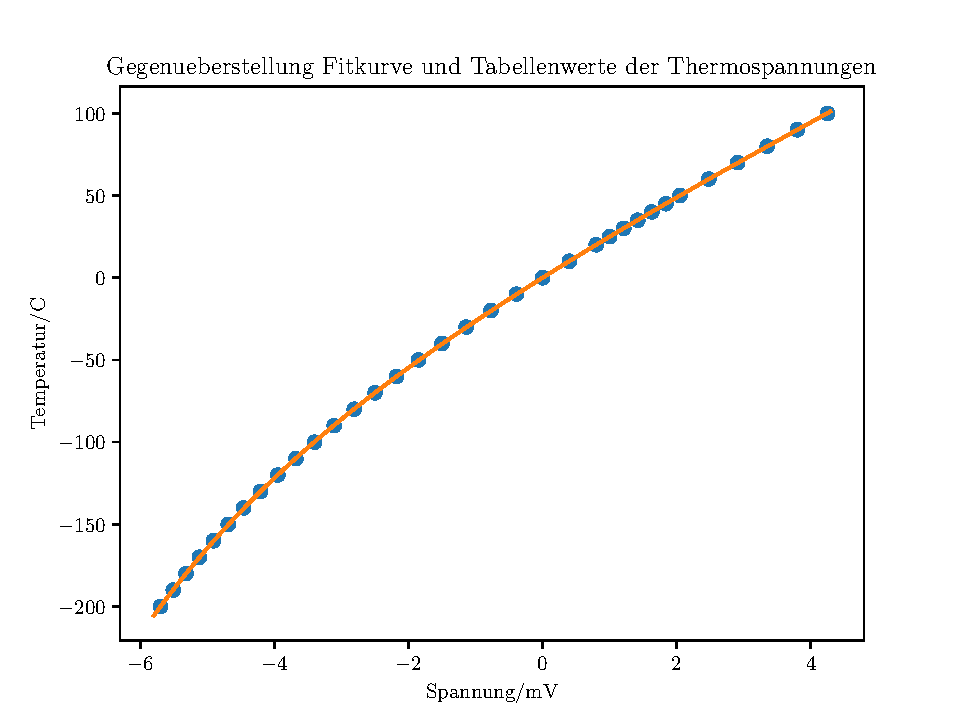
\includegraphics[scale=0.7]{temp_fit.pdf}
  \caption{Temperaturfit der Temperaturspannung}
  \label{temp}
\end{figure}

Aus den Messwerten direkt ersichtlich ist das negative Vorzeichen der Hall-Konstante, woraus die Dotierung als n-Dotierung identifiziert werden kann.

Die Verläufe der Größen $R_H$, $n$ und $\rho$ sind in den Abbildungen \ref{hall} bis \ref{n} logarithmisch gegenüber $\frac{1}{T}$ dargestellt. Für die Berechnung des spezifischen Widerstands wurde dabei ein konstanter Wert von $f=0.97$ für den Korrekturfaktor verwendet. 

\begin{figure}[htbp] 
     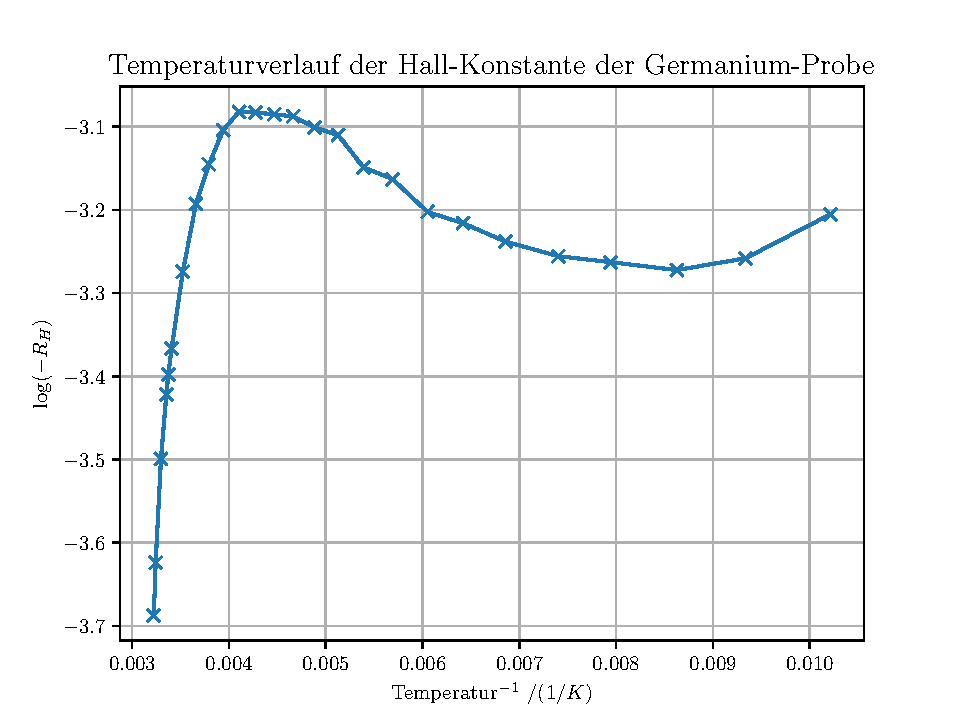
\includegraphics[scale=0.7]{temp_hall.pdf}
  \caption{Temperaturverlauf der Hall-Konstante}
  \label{hall}
\end{figure}

\begin{figure}[htbp] 
     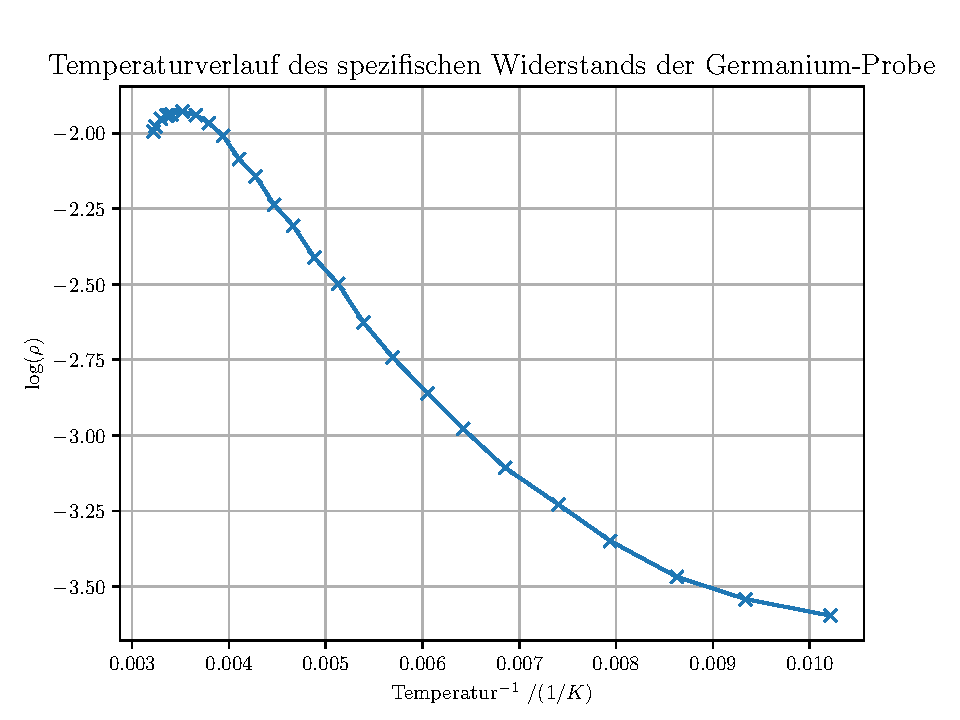
\includegraphics[scale=0.7]{temp_rho.pdf}
  \caption{Temperaturverlauf des spezifischen Widerstands}
  \label{hall}
\end{figure}

\begin{figure}[htbp] 
     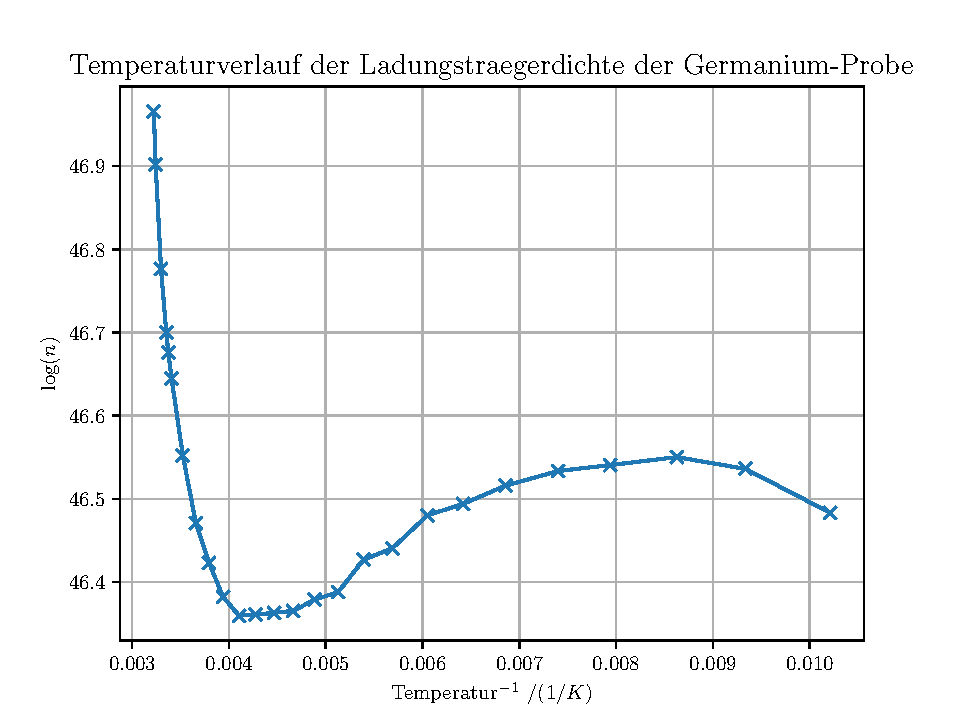
\includegraphics[scale=0.7]{temp_n.pdf}
  \caption{Temperaturverlauf der Ladungsträgerdichte}
  \label{n}
\end{figure}

Wie zu erwarten, nimmt der gemessene spezifische Widerstand linear mit der reziproken Temperatur ab. Die kleine Überhöhung zu Beginn der Kurve ist dabei über die Messungenauigkeiten zu erklären, welche besonders bei den extremen, d.h. sehr hohen und sehr niedrigen Temperaturen zum Tragen kamen. So war der geplante Messwert bei $40^{\circ}C$ mit dem Heizer nicht ganz zu erreichen, da ein Fehler im Vakuum der Messanordnung vorlag.  

Die gemessene Hall-Konstante wie auch die Ladungsträgerdichte weisen im hohen Temperaturbereich das charakteristische exponentielle Verhalten auf und steigt rasant an. Im mittleren Temperaturbereich erwarten wir in beiden Schaubildern einen konstanten Verlauf, wohingegen wir einen leichten Anstieg messen. Dies ist physikalisch unsinnig, da bei niedrigerer Temperatur natürlich auf keinen Fall mehr Ladungsträger im Leitungsband vorhanden sein sollten, sondern die Ladungsträgerdichte aufgrund der Störstellenerschöpfung konstant sein sollte. Hin zu besonders niedrigen Temperaturen sinkt die gemessene Ladungsträgerdichte wiederum ab, was aufgrund der Anhebung von immer weniger Elektronen ins Leitungsband auch so zu erwarten war. 
Bei Betrachtung unserer Messwerte muss allerdings auch die sehr hoch aufgelöste Skala beachtet werden, sodass unsere Schwankungen im konstant erwarteten Bereich im Vergleich besonders zu den sehr stark steigenden Messwerten im Hochtemperaturbereich nicht sehr stark ins Gewicht fallen. Da weiterhin die Tief- und Mitteltemperaturmessung mit sehr schnell steigenden Temperaturen durchgeführt wurden, sind die Messwerte mit Vorsicht zu genießen und weisen vermutlichen einen hohen Fehler auf.

Aus den Messergebnissen kann man weiterhin noch die Beweglichkeit der Elektronen in Germanium berechnen. Es gilt nämlich für die Leitfähigkeit:

\begin{align}
\sigma=ne\mu
\end{align}

Daraus folgt für die Beweglichkeit:

\begin{align}
\mu=\frac{1}{ne\rho}
\end{align}

Die Beweglichkeit ist ebenfalls temperaturabhängig und in Abbildung \ref{mu} doppelt logarithmisch dargestellt.

\begin{figure}[htbp] 
     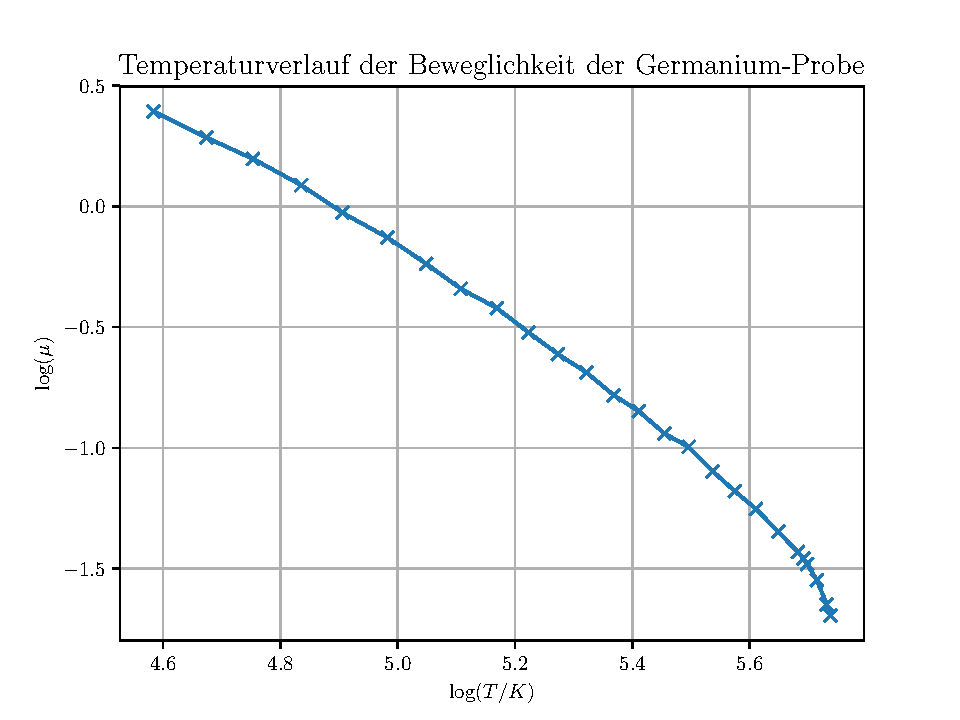
\includegraphics[scale=0.7]{temp_mu.pdf}
  \caption{Temperaturverlauf der Beweglichkeit}
  \label{mu}
\end{figure}

Hier sehen wir den erwarteten konstanten Verlauf der Beweglichkeit, welche proportional zur Temperatur abnimmt. Dies lässt sich gut mit dem erwarteten Verlauf in Verbindung setzen, da die Beweglichkeit der Ladungsträger aufgrund steigender thermischer Anregung und den damit verbundenen Stößen mit den Ionenrümpfen mit der Temperatur abnimmt. 
\section{Zusammenfassung/Fazit}
Im durchgeführten Versuch konnte der Hall-Effekt sehr anschaulich gezeigt und auf die Bandstruktur von Halbleitern angewandt werden. Dabei waren sowohl die angewandten experimentellen Methoden als auch die gezeigten theoretischen Zusammenhänge mit zufriedenstellendem Erkenntnisgewinn verbunden. Die Van-der-Pauw-Methode stellte dabei eine interessante Alternative zur Vermessung des Hall-Effekts dar. Besonders die vermessenen Temperaturverläufe der Ladungsträgerdichte und der Beweglichkeit sorgten für eine willkommene Veranschaulichung der bekannten theoretischen Verläufe. Die Bestimmung der Bandlücke war nur sehr fehlerbehaftet möglich, die Idee dahinter konnte jedoch vermittelt und beschrieben werden.

\bibliography{Literaturverzeichnis}



\end{document}
